\documentclass{standalone}
\usepackage{tikz}
\usetikzlibrary{matrix, positioning, shapes, arrows, calc}

\tikzset{>=latex}

\begin{document}

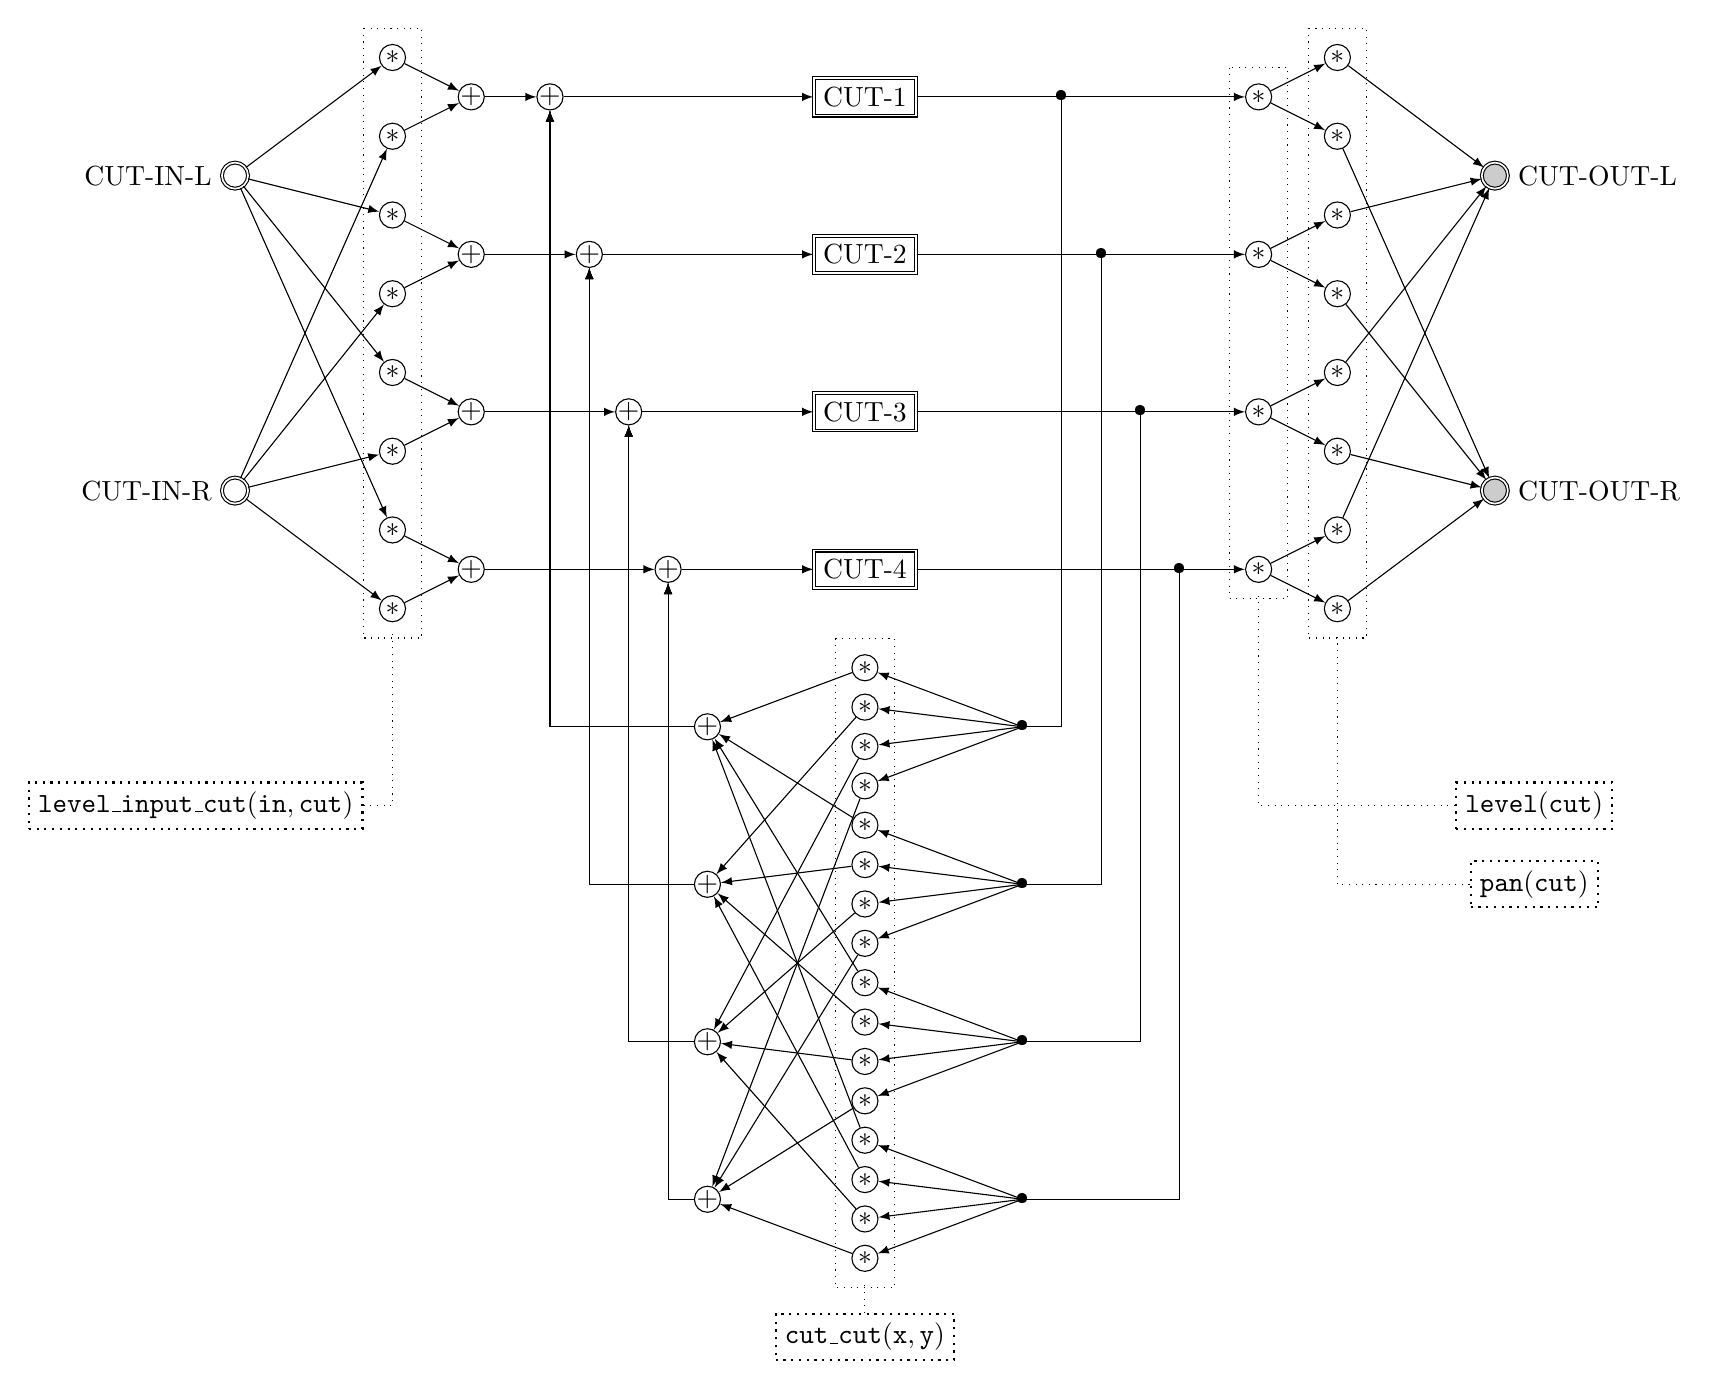
\begin{tikzpicture}

\tikzstyle{input}=[draw=black, circle, double, minimum size=1]
\tikzstyle{output}=[draw=black, circle, double, minimum size=1, fill=gray!40]
\tikzstyle{mul}=[draw=black, circle, minimum size=1, label=center:$\ast$]
\tikzstyle{add}=[draw=black, circle, minimum size=1, label=center:$+$]
\tikzstyle{or}=[draw=black, circle, minimum size=1, label=center:$|$]
\tikzstyle{param}=[draw=black, rectangle, dotted, thick]
\tikzstyle{bus}=[draw=black, rectangle, double]


% inputs
\node [input, label=left:CUT-IN-L] (in-l) at (0, 10) {};
\node [input, label=left:CUT-IN-R] (in-r) at ($(in-l) - (0, 4)$) {};

\node [mul] (in-l-mul-1) at ($(in-l) + (2, 1.5)$) {};
\node [mul] (in-r-mul-1) at ($(in-l-mul-1) +(0, -1)$) {};
\node [mul] (in-l-mul-2) at ($(in-r-mul-1) +(0, -1)$) {};
\node [mul] (in-r-mul-2) at ($(in-l-mul-2) +(0, -1)$) {};
\node [mul] (in-l-mul-3) at ($(in-r-mul-2) +(0, -1)$) {};
\node [mul] (in-r-mul-3) at ($(in-l-mul-3) +(0, -1)$) {};
\node [mul] (in-l-mul-4) at ($(in-r-mul-3) +(0, -1)$) {};
\node [mul] (in-r-mul-4) at ($(in-l-mul-4) +(0, -1)$) {};

\draw [->] (in-l) -- (in-l-mul-1);
\draw [->] (in-l) -- (in-l-mul-2);
\draw [->] (in-l) -- (in-l-mul-3);
\draw [->] (in-l) -- (in-l-mul-4);
\draw [->] (in-r) -- (in-r-mul-1);
\draw [->] (in-r) -- (in-r-mul-2);
\draw [->] (in-r) -- (in-r-mul-3);
\draw [->] (in-r) -- (in-r-mul-4);

% cuts
\node [add] (cut-in-1) at ($(in-l-mul-1) + (1, -0.5)$) {};
\node [add] (cut-in-2) at ($(cut-in-1) + (0, -2)$) {};
\node [add] (cut-in-3) at ($(cut-in-2) + (0, -2)$) {};
\node [add] (cut-in-4) at ($(cut-in-3) + (0, -2)$) {};


% feedback!
\node [add] (cut-in-fb-1) at ($(cut-in-1) + (1, 0)$) {};
\node [add] (cut-in-fb-2) at ($(cut-in-2) + (1.5, 0)$) {};
\node [add] (cut-in-fb-3) at ($(cut-in-3) + (2, 0)$) {};
\node [add] (cut-in-fb-4) at ($(cut-in-4) + (2.5, 0)$) {};
\foreach \i in {1,...,4}
{
	\node [bus] (cut-\i) at ($(cut-in-\i) + (5, 0)$) {CUT-\i};
	\draw [->] (in-l-mul-\i) -- (cut-in-\i);
	\draw [->] (in-r-mul-\i) -- (cut-in-\i);
	\draw [->] (cut-in-\i) -- (cut-in-fb-\i);
	\draw [->] (cut-in-fb-\i) -- (cut-\i);
	\node [mul] (cut-out-mul-\i) at ($(cut-\i) + (5, 0)$) {};
	\draw [->] (cut-\i) -> (cut-out-mul-\i);
	\node (cut-out-fb-split-\i) at ($(cut-\i) + (2 + \i*0.5, 0)$) {\textbullet};
}

\node (fb-in-1) at ($(cut-4) + (2, -2)$) {\textbullet};
\node (fb-in-2) at ($(fb-in-1) + (0, -2)$) {\textbullet};
\node (fb-in-3) at ($(fb-in-2) + (0, -2)$) {\textbullet};
\node (fb-in-4) at ($(fb-in-3) + (0, -2)$) {\textbullet};

\foreach \i in {1,...,4}
{
	\draw (cut-out-fb-split-\i.center) |- (fb-in-\i.center);
	\node [mul] (fb-\i-1) at ($(fb-in-\i) + (-2, 0.75)$) {};
	\node [mul] (fb-\i-2) at ($(fb-in-\i) + (-2, 0.25)$) {};
	\node [mul] (fb-\i-3) at ($(fb-in-\i) + (-2, -0.25)$) {};
	\node [mul] (fb-\i-4) at ($(fb-in-\i) + (-2, -0.75)$) {};
	\node [add] (fb-out-\i) at ($(cut-\i) + (-2, -8)$) {};
	\foreach \j in {1,...,4} 
	{
		\draw [->] (fb-in-\i.center) -- (fb-\i-\j);
	}
}
\foreach \i in {1,...,4}
{
	\foreach \j in {1,...,4} 
	{
		\draw [->] (fb-\j-\i) -- (fb-out-\i);
		\draw [->] (fb-out-\i) -| (cut-in-fb-\i);
	}
}

% outputs
\foreach \i in {1,...,4}
{
	\node [mul] (cut-out-l-mul-\i) at ($(cut-out-mul-\i) + (1, 0.5)$) {};
	\node [mul] (cut-out-r-mul-\i) at ($(cut-out-mul-\i) + (1, -0.5)$) {};
	\draw [->] (cut-out-mul-\i) -- (cut-out-l-mul-\i);
	\draw [->] (cut-out-mul-\i) -- (cut-out-r-mul-\i);
}
\node [output, label=right:CUT-OUT-L] (cut-out-l) at ($(cut-out-l-mul-1) + (2, -1.5)$) {};
\node [output, label=right:CUT-OUT-R] (cut-out-r) at ($(cut-out-l) + (0, -4)$) {};
\foreach \i in {1,...,4}
{
	\draw [->] (cut-out-l-mul-\i) -- (cut-out-l);
	\draw [->] (cut-out-r-mul-\i) -- (cut-out-r);
}

% labels 
\draw [dotted] ($(in-l-mul-1.north west)+(-0.25,0.25)$)  rectangle ($(in-r-mul-4.south east)+(0.25,-0.25)$);
\node [param] (level-input-cut) at ($(in-r) + (-0.5, -4)$) {$\tt{level\_input\_cut(in,cut)}$};
\draw [dotted] (level-input-cut) -| ($(in-r-mul-4) + (0, -0.3)$);

\draw [dotted] ($(cut-out-mul-1.north west)+(-0.25,0.25)$)  rectangle ($(cut-out-mul-4.south east)+(0.25,-0.25)$);
\node [param] (level) at ($(cut-out-r) + (0.5, -4)$) {$\tt{level(cut)}$};
\draw [dotted] (level) -| ($(cut-out-mul-4) + (0, -0.3)$);

\draw [dotted] ($(cut-out-l-mul-1.north west)+(-0.25,0.25)$)  rectangle ($(cut-out-r-mul-4.south east)+(0.25,-0.25)$);
\node [param] (pan) at ($(cut-out-r) + (0.5, -5)$) {$\tt{pan(cut)}$};
\draw [dotted] (pan) -| ($(cut-out-r-mul-4) + (0, -0.3)$);

\draw [dotted] ($(fb-1-1.north west)+(-0.25,0.25)$)  rectangle ($(fb-4-4.south east)+(0.25,-0.25)$);
\node [param] (cut-cut) at ($(fb-4-4) + (0, -1)$) {$\tt{cut\_cut(x,y)}$};
\draw [dotted] (cut-cut) -- ($(fb-4-4) + (0, -0.3)$);


\end{tikzpicture}
\end{document}













